%!TEX root = ../article.tex

\section{Analyzing Color Mixing Perception}
\label{sec:results}
%
The users were given always the same briefing when they arrived at the user study test site: it was
explained the motivation behind the master thesis, the goals which were expected for this phase of
the study and what was expected for them to execute. The user was told that \ul{"there are no
pre-defined correct and wrong answers to each question, this test was designed to test the general
color mixing capabilities of the majority of the users"}. The user study was self-contained, in the
sense that every other relevant information and instruction was in the interface, adapted for each
test phase, so it was not given any physical artifacts giving instructions. \par
%
In order to collect a larger amount of users (either for the laboratory or online study), we had to
spread the study both by \emph{word-of-mouth} and across some online platforms. We have opted for
spreading the study across social networks like Facebook\textsuperscript{\textregistered} or
StumbleUpon. However, we found that gathering the laboratory users was a tough job to do, since many
prospective users were not willing to fulfill the study. Thus, we explored a \emph{Reddit} subthread
called "Sample Size", which exists to disseminate user studies across the internet, which provided
159 new visitors to our webpage. \par
%
We collected a \textbf{total amount of 477 users} which interacted with our study and fulfilled, at
least, until the Color Vision Deficiencies Test Phase. However, only \textbf{259 users went on to
the core phase of the study}, representing \textbf{54.29\%} of the total amount, giving at least one
answer on the set of 32 questions; the 218 users that did not leave an answer amount to
\textbf{45.71\%}. There were \textbf{28 users who performed the entire study on the laboratory trials}.
On the other hand, there were \textbf{231 users which carried out the study online}. The data presented
and used in this dissertation document was gathered during roughly two months, from 15\textsuperscript{th}
of April until 8\textsuperscript{th} of June. \par
%
Note that the main data to be analyzed is the one obtained in the laboratory environment, being the
online data only the corroboration of the main data. Each chromaticity diagram presented in this Section,
shows a \textbf{black filled dot} which corresponds to the ideal answer for each color model, and
\textbf{two black empty dots} which are the blending-basis of questions which have asked for it; the
\textbf{grey dots} represent the answers given by the users, and the black lines represent the union
between each grey dot, forming each answer pair given.
%
\subsection{User Profile}
%
Our user sample is composed by 259 (100\%) users, being \textbf{105 (40.5\%) Females}, \textbf{152
(58.7\%) Males} and a minority of \textbf{2 (0.8\%) Other gendered users}: this sample age can
be characterized as being generally young ($\overline{x} = 29.77$, $\overline{x} = 23$, $s = 40.30$ ),
surprisingly having \textbf{8 users (3.09\%) aged above 60 years old} which could enhance some interesting
differences between age groups. Generally, our users have high academic qualifications, representing
\textbf{66.02\% of all users (Bachelor, Master and Doctoral Degrees)}, being \textbf{38 (14.67\%) users
qualified with College degree}, \textbf{47 (18.15\%) have a High-School degree} and only \textbf{3 (1.16\%)
subjects do not presented any academic degree}. Between the laboratory and online environment, the
distribution of users remains with the same proportions: more male users than females, mostly aged
between 20 and 29 years old (60.71\%) and the majority having a superior academic degree (46.43\% BSc
and 35.71\% MSc). From the entire user set, \textbf{215 (83.01\%) of them have Portuguese nationality},
\textbf{217 (83.78\%) live in Portugal} currently and \textbf{216 (83.40\%) speak Portuguese}; the second
most influent group of users are the ones from english-speaking countries (United Kingdom, United States
of America, and others). Other minor users which contributed to our survey came from Turkey, France, New
Zealand, Sweden or even Antarctica (among others) - \textbf{these countries represent only 5.41\%}.\par

\subsection{Color Models}
%
Since the colors obtained in the color slider from the \ul{Core Phase} indicate values for the HSV Color
Model, the values were converted from HSV to CIE-XYZ Color Model. Thus, we can produce color blends in
every studied color model (HSV, RGB, CMYK, CIE-L*a*b* and CIE L*C*h*) and ensure that colors obey to the
same common standard; also, this is specially important to produce Chromaticity Diagrams where colors are
mapped according to a set of XYZ primitives. Afterwards, every resulting blending is compared to the
pre-calculated value for each color model, and the euclidean distance to the latter value is stored
for statistical analysis. It was this distance which we had considered when analyzing the relationship
between the users’ expectations and each color model. \par
%
The Color Model which presented the lowest mean value for distances was the CMYK Color Model
($\overline{x} = 0.10$), followed by HSV, RGB and CIE-L*a*b* (all with $\overline{x} = 0.14$), being
CIE-L*C*h the model which has the highest calculated distances ($\overline{x} = 0.20$). Consistently,
the color model which has the lowest variance and range of answers is the CMYK ($s^2 = 0.001$, $range
= 0.14$), opposed to the HSV ($s^2 = 0.006$, $range = 0.26$). Performing a \emph{Wilcoxon} Test, we
conclude that there are no statistically significant differences between the laboratory distances and
online ones ($p < 0.05$), which means that the online results corroborate the laboratory ones.
%
\subsubsection{HSV Color Model}
%
The questions which have shorter distances are number 11 (given orange and expected green and magenta),
number 17 (given green, expected blue and yellow) and number 6 (given orange, expected red and yellow),
with mean values of $\overline{x} = 0.0587$, $\overline{x} = 0.0683$ and $\overline{x} = 0.0741$,
respectively. On the other hand, we found that the questions which generate the worst results are number
2 (given magenta, expected red and blue), number 13 (given a shade of blue, expected blue and cyan) and
number 10 (given a shade of blue, expected green and magenta), with correspondent mean values
$\overline{x}_{2} = 0.2173$, $\overline{x}_{13} = 0.2713$ and $\overline{x}_{10} = 0.3$. \par
%
When comparing the results from the HSV color model with other color models' results, we detected some
statistically significant differences with other models: performing a \emph{Wilcoxon} Test ($p < 0.05$), we can
infer that HSV does have statistically significant differences with CIE-L*C*h*, CMYK, RGB and CIE-L*a*b*
in the majority of questions. Due to the fact that there are color primitives which are opposed in the
HSV hue circle, there are in this study three pairs of colors which blend onto two possible colors: pairs
Red-Cyan, Green-Magenta and Blue-Yellow. By placing these questions, we intended to understand which side
the user would tend to follow when asked to indicate the blending-basis. In this article, we analyze just
one of these. \par
%
The diagram of Figure \ref{fig:hsv_analysis} contains the three top and bottom-valued questions, disposed
on top of an interval $[0 ; 0.5]$ of differences. Each question is mapped according to its mean value for
distance to the ideal HSV Color Model response, while is accompanied by the range of values which compose
its answers.
%
\begin{figure}[!htbp]
  \centering
  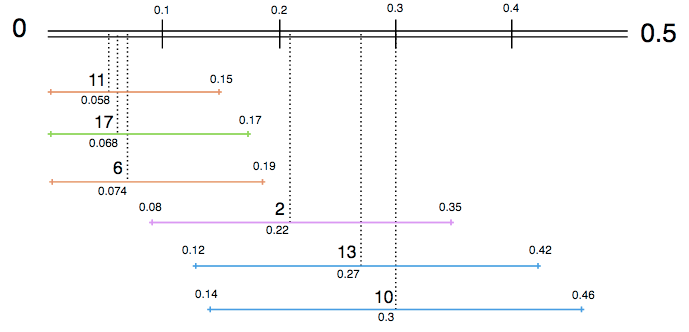
\includegraphics[width=0.4\textwidth]{images/hsv_questions_analysis.png}
  \caption{Best and Worst Questions, according to HSV Color Model.}
  \label{fig:hsv_analysis}
\end{figure}
%
\subsubsection{CIE-L*C*h* Color Model}
%
This model has the highest mean value on laboratory and online environment, and the highest standard
deviation, range and variance exclusively on the online environment. The three questions which have
shorter distances are number 6 (given orange, expected red and yellow), number 5 (given a shade of
red, expected red and magenta) and number 2 (given magenta, expected red and blue). The mean values
distances for this questions were, contrary to the previous color model, are all values above $0.1$
(a quite high value in the scale which results are presented), that could represent a significant
change in the resultant color. \par
%
The model which CIE-L*C*h* has most statistically significant differences with is CMYK, with eleven
questions, according to the \emph{Wilcoxon} Test ($p < 0.05$). Question 6 presented again a constant
top value for the mean value, on this model, which leads us to formulate the theory that the
\textbf{orange color is commonly used and mixed by the users}. On the other hand, question 10 kept
having one of the worst mean value ($\overline{x}_{10} = 0.2557$), strengthening the theory that
\textbf{blue shades and tones will probably wild worst results, due to the fact that it is the color
which human have less descriptive power}. \par
%
The diagram of Figure \ref{fig:lch_analysis} contains the three top and bottom-valued questions,
disposed on top of an interval $[0 ; 0.5]$ of differences.
%
\begin{figure}[!htbp]
  \centering
  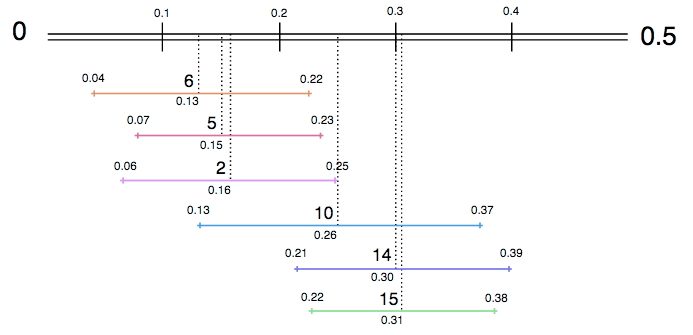
\includegraphics[width=0.4\textwidth]{images/lch_questions_analysis.png}
  \caption{Best and Worst Questions, according to CIE-L*C*h* Color Model.}
  \label{fig:lch_analysis}
\end{figure}
%
\subsubsection{CMYK Color Model}
%
This model is, by far, the one which presents the best results: it has the lowest mean value of
distances ($\overline{x}_{lab} = 0.10$, $\overline{x}_{online} = 0.09$), lowest standard deviation
($s_{lab} = 0.04$, $s_{online} = 0.04$), the lowest range of values ($range_{lab} = 0.14$,
$range_{online} = 0.11$) and, finally, the lowest variance value ($s^2_{lab} = 0.001$, $s^2_{online}
= 0.001$). The three questions which have shorter distances are number 17 (given a green, expected
cyan and blue), number 6 (given orange, expected red and yellow) and number fifteen (given a shade
of green, expected blue and yellow). The mean values distances for this questions were $\overline{x}_{17}
= 0.0452$, $\overline{x}_{6} = 0.0577$ and $\overline{x}_{15} = 0.0625$ which, contrary to the
previous color model, are all values \ul{below $0.1$}, that does not represent a significant change
in the resultant color. \par
%
Question 17 presented consistently another low value: along with question 3 and 15, these presented
different \ul{shades of green} and all had yielded favorable results. This may lead us to form another
conclusion: \textbf{questions which presented shades of green color may produce better results, according
to users' expectations}. This is consistent with the fact that \textbf{humans have more descriptive power
in the green zone of the spectrum, due to the amount of cones which exist in the human eye}. \par
%
The questions which yielded \textbf{better results are majorly related to primitives of the CMYK color
model}. This success could be related to the fact that \textbf{people tend to formulate mental models of
color based on ink mixing in childhood} \cite{Gossett2004}, mostly associating it to CMYK Color Model
without even knowing it. \par
%
\begin{figure}[!htbp]
  \centering
  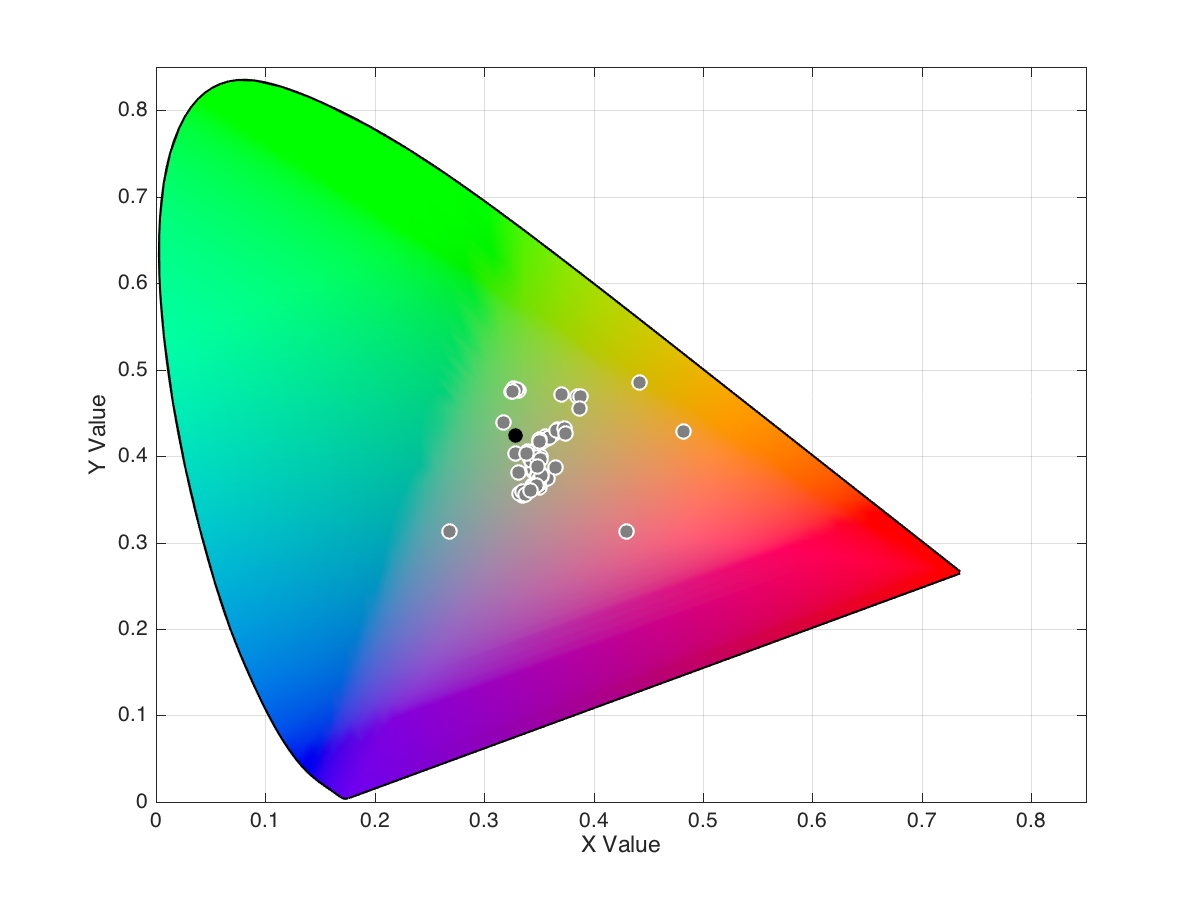
\includegraphics[width=0.35\textwidth]{images/17_online_CMYKresponses.png}
  \caption{Online: Question 17, Regular users, mixed in CMYK.}
  \label{fig:onlinecmykregular_17}
\end{figure}
%
Figure \ref{fig:onlinecmykregular_17} show the results for Question 17, the question with closer
distances. The diagram of Figure \ref{fig:cmyk_analysis} contains the three top and bottom-valued questions, disposed on top of an interval $[0 ; 0.5]$ of differences.
%
\begin{figure}[!htbp]
  \centering
  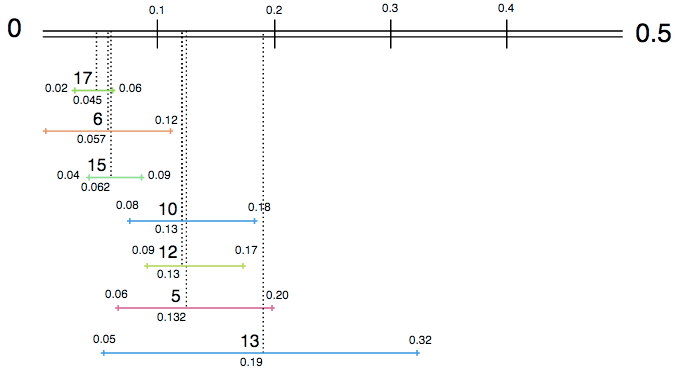
\includegraphics[width=0.4\textwidth]{images/cmyk_questions_analysis.png}
  \caption{Best and Worst Questions, according to CMYK Color Model.}
  \label{fig:cmyk_analysis}
\end{figure}
%
\subsubsection{RGB Color Model}
%
This color model is complementary to the CMYK color model. Feedback collected from the users was such
that, sometimes, the users which knew how to blend in subtractive color models, tended to be confused
and tried to mix additive color models, also. Based on the results collected from the laboratory users,
we can tell that the results from this color model are quite similar to CMYK results: RGB has one of
the lowest mean value of distances ($\overline{x}_{lab} = 0.14$, $\overline{x}_{online} = 0.12$) and
one of the lowest standard deviations ($s_{lab} = 0.05$, $s_{online} = 0.04$ equal to $s_{CMYK-online}$).
The three questions which have shorter distances are number number 6 (given orange, expected red and
yellow), number 9 (given a shade of green, expected green and cyan) and 17 (given a green, expected
cyan and blue). The mean values distances for this questions were $\overline{x}_{6} = 0.0777$,
$\overline{x}_{9} = 0.1005$ and $\overline{x}_{17} = 0.1030$. \par
%
When comparing the results from the RGB color model, the majority of users did reveal lack of knowledge
in mixing the colors according to an additive color model, as they tended to mix colors according to the
CMYK color model. However, this color model has a high degree of compatibility with every other model,
excepting CMYK: performing a Wilcoxon Test ($p < 0.05$), we can infer that RGB does not present
statistically significant differences with HSV, CIE-L*a*b* and with CIE-L*C*h* in 10 questions, while
presenting statistically significant differences with CMYK in 13 questions. \par
%
Relating to the fact that people either tend to blend colors in an additive or subtractive way, we can
compare the results from this color model with CMYK model and state that \textbf{users tend to formulate
subtractive mental models of color blending}. However, \textbf{there is room for further investigation,
to fully understand if users are influenced by additive color models or subtractive ones}. The diagram
of Figure \ref{fig:rgb_analysis} contains the three top and bottom-valued questions.
%
\begin{figure}[!htbp]
  \centering
  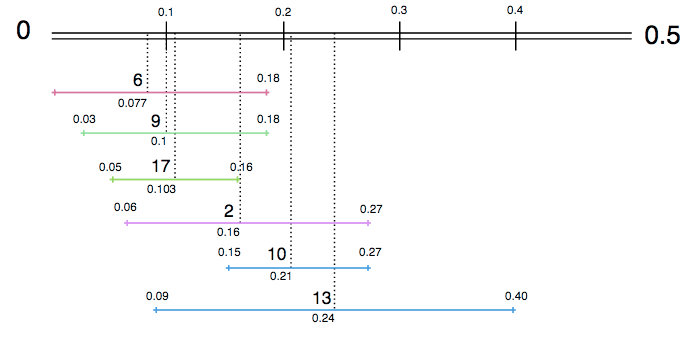
\includegraphics[width=0.4\textwidth]{images/rgb_questions_analysis.png}
  \caption{Best and Worst Questions, according to RGB Color Model.}
  \label{fig:rgb_analysis}
\end{figure}
%
\subsubsection{CIE-L*a*b* Color Model}
%
This color model has results very similar to CMYK and RGB, since its descriptive statistics have comparable
values to this model. The three questions which have shorter distances are number number 6 (given orange,
expected red and yellow), 17 (given a green, expected cyan and blue) and number 9 (given a shade
of green, expected green and cyan), which are exactly the same as before. The mean values distances for
this questions were $\overline{x}_{6} = 0.0509$, $\overline{x}_{17} = 0.1130$ and $\overline{x}_{9} = 0.1142$. \par
%
Since the CIE-L*a*b* conveys the entire set of perceived by the human eye, it \textbf{explains why the
results associated with this color model are so close to others which yield the best results}. The diagram
of Figure \ref{fig:lab_analysis} contains the three top and bottom-valued questions.
%
\begin{figure}[!htbp]
  \centering
  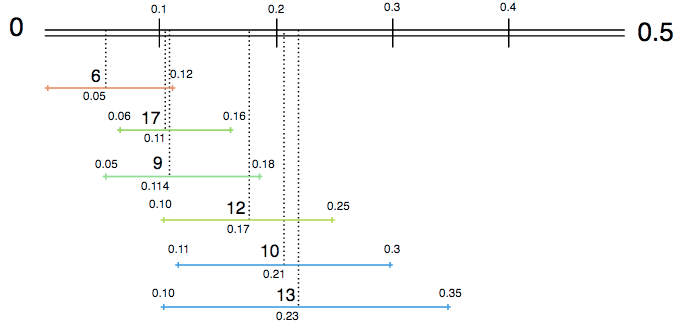
\includegraphics[width=0.4\textwidth]{images/lab_questions_analysis.png}
  \caption{Best and Worst Questions, according to CIE-L*a*b* Color Model.}
  \label{fig:lab_analysis}
\end{figure}
%
\subsection{Color Blending Expectation}
%
Besides asking our users to indicate us the two primitives which composed a color blending of two colors,
we intended to go further: \textbf{comprehend if more than detecting two colors of a mixture, a user
is capable of mentally blend two given colors and indicate us its results}. \par
%
We end up concluding that the question which constantly had best results among all color models was the
blending of red and yellow to create orange. However, these results represent much
higher distances to the ideal answer in any color model, than when given the user the resulting color of
the blending. This fact could accuse that \textbf{it is harder for the users to detect the result of a
color blend, when two blending basis are given, than when the resulting color is given}, even for the
orange color blending which produced very good results in the previous analysis. \par
%
Contrary to questions in which the user was asked to indicate the blending basis, \textbf{the color model
which has the worst results is the HSV Color Model} ($\overline{x}_{HSV} = 0.18$) while the one which has
\textbf{the shortest mean distance value continues to be CMYK, along with CIE-L*a*b*} ($\overline{x} = 0.13$).
%
\subsection{Color Blendings \& Naming}
%
Since the creation of an entire study to ascertain this subject was out of the scope of this master
thesis, we used the Color Survey\footnote{Color Survey Results. Available at:
\url{blog.xkcd.com/2010/05/03/color-survey-results/}. Last accessed on October 17th, 2016.} which the web
page XKCD conducted, to study which were the most common RGB color triples among users. They performed
roughly more than 222 000 user sessions to ascertain color naming, producing a map which shows the
dominant names attributed to RGB colors over the faces of RGB cube; they also produced a file comprised
of 196 608 RGB triplets, grouped by \textbf{Color Bins}. We decided to use it given its large sample size,
and it was executed with a great amount of users which can verify it. We also found great compatibility
between this survey and ours, since the values in the first were also presented in its maximum value of
saturation. \par
%
The idea was to compare our answers with each color bin, creating a mapping between our users' values
and commonly-used names; to speed up the computation of the comparisons, each color bin was drawn and
the smallest polygon formed by the set of triplets of each bin was used to compare the values. There
were six questions which presented as the result of a color mixture, either one of the following
primary colors; what we intended to know is if the users are capable of creating color blendings
which result in these colors. For the sake of simplification, in this document we will only present
the analysis of creating \ul{Red based on Magenta and Yellow}, and \ul{Green based on Cyan and Yellow}.
%
\subsubsection{Magenta + Yellow = Red}
%
The laboratory users did focus their answers on \textbf{orange, green, blue and even red hue}; moreover,
these results were similar among the online users and did not demonstrated a consensual answer pair.
Additionally, five laboratory users (from thirteen which indicated a pair of two answers - $38.46\%$ of the users)
and forty-two online users (from sixty-two - $67.74\%$ of the users) indicated, at least, one time the red color
as an answer. These evidences lead us to believe that \textbf{the users do not know how to create a red color
based on other primary colors}. \par
%
Since we have produced the mapping between given values and color bins, we can perform a qualitative
analysis of each answer pair's colors names while comparing it to the expected ones. The expected pair was
\ul{Magenta-Yellow}: among 62 answers from the online users to question 8, \textbf{we conclude that the colors
Magenta and Yellow were among the least indicated ones}, being Magenta indicated four times and five times. The
most repeated color was Red, being indicated more than
70 times: there were 31 answer-pairs ($50\%$) which contained the color Red twice! When given by the user, the
Magenta was combined with Green and Red, while Yellow was combined with Red, Green and Blue; however, the specific
pair Magenta-Yellow was never indicated.
%
\subsubsection{Cyan + Yellow = Green}
%
Both the laboratory and online users provided their answers on similar pairs, comprised between \textbf{blue shades
and yellow ones}; the most repeated color pairs were, in fact, Blue shades combined with tones of green and yellow,
as observable on Figure \ref{fig:greenblend_1}. Additionally, only two laboratory users (from twenty-three which
indicated a pair of two answers - $8.70\%$ of the users) and six online users (from seventy-one - $8.45\%$ of the
users) indicated an answer pair which did not even nearly approximate to the desired hues. \par
%
The expected pair was \ul{Cyan and Yellow}: among 71 answers from the online users to question 17, \textbf{we conclude
that the color Yellow was among the least indicated ones}; however, users have diverged a little when indicating the cyan
color, since \textbf{the users have answered with colors varying between Blue, Navy-Blue, Sky-Blue, Light-Blue and
Teal}, with frequencies of 37, 11, 3, 1 and 1 respectively, while Cyan was only referred 4 times. Though, users
have referenced a lot more times the Green color, which is the presented one: 77 times to be more precise, with
\textbf{53 answer-pairs formed with a Blue shade and Green} ($75\%$ of the totality of pairs) and 10 pairs which
contained the Green color twice. If analyzed, the CIE Chromaticity Diagram in Figure \ref{fig:greenblend_1}
consolidates this idea, revealing the dispersion of blue derived colors' usage, but a slight concentration of
answers in the neighborhood of Green and Yellow. Regarding the latter, it was combined 4 times with blue shades
which is another indicator that \textbf{users presented strong Blue-Green/Yellow blending capabilities}.
%
\begin{figure}[!htbp]
  \centering
  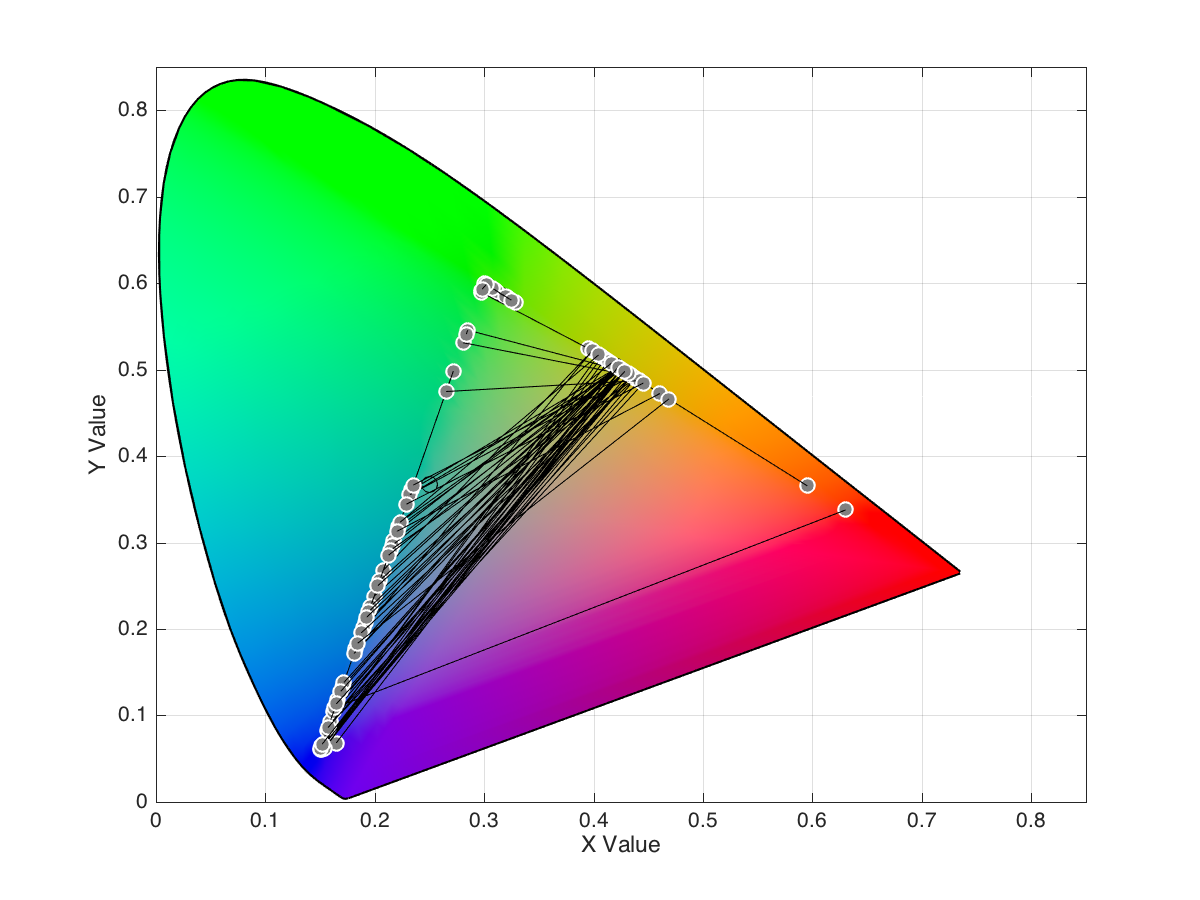
\includegraphics[width=0.35\textwidth]{images/17_online_regularUsers.png}
  \caption{Online: Question 17, Regular users.}
  \label{fig:greenblend_1}
\end{figure}
%
\subsection{Color Blending Effort}
%
We have collected from the users the easiness of blending two shades of colors, when concluding each
answer. This easiness is reflected in an numerical scale, ranged from one to five, being one the hardest
level of effort, and five the easiest level of effort. The results are in agreement with the ones collected
and concluded before: the \textbf{blending of Red-Green resulting in Yellow}, \textbf{blending of Red-Yellow
and Green-Magenta, both resulting in Orange} and the \textbf{blending of Cyan-Yellow resulting in Green} were
the mixtures which, according to the users' answers, had the lowest effort of blending, consequently the
highest rating of easiness; particularly for the mixture of Red and Yellow, resulting in Orange, it provides
the best results in both question types. Contrary, the questions which had the lowest results were almost always the ones in which the user was inquired about the result of given blending basis. \par
%
It is interesting to observe that the results for the generality of questions encircle the rating of 2 and 3
in the interval $[1 ; 5]$, which could indicate that \textbf{apart from the obvious color blendings which
proved to yield the best results, all the other blendings show nor an easy or hard level of effort to mix
the basis}. These results are confirmed by the online responses, by running a Friedman Test which indicates
us that there are no statistically significant differences ($p < 0.05$) when comparing the results from the
laboratory environment, with the online results.
%
\subsection{Demographic Results}
%
We performed a set of statistic tests to realize if there is some kind of connection between the
demographic information of our users and the answers given by them, for example a relation between
the answers given by the male and female users, or even if the younger users interpret the color
blendings differently from the older ones. \par
%
We have separated the users among some demographic groups: regarding the age division we have created
six groups (\textbf{users aged below 20 years, aged between 20-29, 30-39, 40-49, 50-59, and above 60 years}),
and for the gender we have divided the dataset according to \textbf{female, male and other gendered users}.
These groups were, then, iterated by question, performing a \emph{Spearman's} Rank-Order Correlation test
between the ages and genders, with the answers. To test the differences between age groups, we have executed
a \emph{Wilcoxon} Signed-rank Test ($p < 0.05$) in order to detect significant differences which exist, between results for each color model, by age group. \par
%
The test reveals that the age group which was always present in each difference, for the selected questions,
was \textbf{the users aged between 40 and 49 years}. However, \textbf{there is insufficient information for
us to confirm that this age group presents much different values from the others}, since these questions
present a minority of the sample. It is also \textbf{not possible to affirm that there are significant
differences between all age groups}, because there are more questions which do not present any difference
\emph{per} color model and the analyzed differences include only a subset of all age groups. Hence,
\textbf{we did not found relevant differences between age groups}. \par
%
Equally to age groups' analysis, we have executed a Wilcoxon Signed-rank Test ($p < 0.05$) in order to
detect significant differences which exist, between results for each color model, by gender group. The
test reveals that there is a mild difference between the results from the Female gendered users, and
the Male ones. It is not an absolute difference, since \textbf{not every question had presented significant
differences between gender groups}; it is \textbf{not possible to formulate a conclusion about which gender
generates the wider or closer distances to the ideal answer (according to each Model)}, since there is no
visible pattern about this subject. There were no significant differences between female
or male users, and the \emph{other} gendered users: this could due to the lack of a significant user sample
relating the later gender.
%
\subsection{Guidelines for Color Blending Usage}
%
The following list enumerates a set of guidelines which we are able to formulate, based on our user study,
about the usage of color blending when sketching visualizations:
%
\begin{enumerate}
  \setlength\itemsep{0.01em}
  \item To maximize the compatibility with the user's expectations, the \textbf{chosen} color blends must present Orange shades based on mixing Red and Yellow.
  \item Color blends which present a resulting color of Green are easier for the user.
  \item The Yellow color provides very good results, when blending Red and Yellow.
  \item The CMYK Color Model is the one which has the best results, according to user's expectations.
  \item To maximize the compatibility with the user's expectations, \textbf{avoid} presenting colors which are near Blue shades.
  \item When presenting Red shades, the best blending-basis which generates it is Red and Magenta.
  \item Presenting the resultant color from a given blending, generally, produces better results than asking the user to blend the color according to his mental model of color.
  \item The color model which best resembles the users' expectation is a subtractive one.
  \item If the usage of CMYK Color Model is not desired, the usage of HSV, RGB and CIE-L*a*b* can produce similar results between each other.
  \item Avoid using the CIE-L*C*h* Color Model when blending colors according to the users' expectations.
\end{enumerate}
